\subsection{Waterfall Model}


The waterfall model is another kind of development process. Unlike Scrum, the waterfall model is not an iterative process.  The waterfall model is made up of a series of process-steps. These steps are Requirement specification, Software design, Implementation, Testing and maintenance. When one phase is finished, another should begin - hence the name Waterfall. Using the waterfall model, the developers can never go back up the process-tree - they have to follow the phase-pattern downward\cite{waterfallexplained}.

\begin{figure}[h]
	\centering
		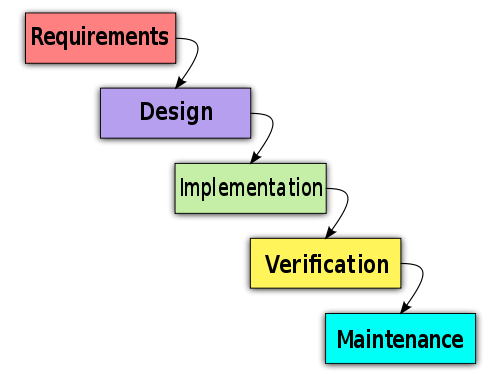
\includegraphics[width=0.8\textwidth]{analysis/waterfall-model.png}
	\label{fig:waterfall-model}
\end{figure}

\subsubsection{Requirement specification}

This is the beginning of a project, and here are all requirements for the project should be 
captured\cite{waterfallexplained}. Typically interviewing the customer helps establish a 
common understanding and foundation for the requirement specification. When a list of 
requirements has been given, they should be analyzed for their 
validity\cite{waterfallexplained}. The result of this phase is the requirement specification 
that can be used in the next phase\cite{waterfallexplained}.
\subsubsection{Software design}


This phase is not a phase used for actual programming. It is here the system is designed, to 
get an overview of what it would look like\cite{waterfallexplained}. The requirement 
specification is studied to help specifying hardware requirements, system requirements and 
overall system architecture\cite{waterfallexplained}.  The results of this phase are 
software design documents that can be used in the next phase\cite{waterfallexplained}.
\subsubsection{Implementation and Unit Testing}


The software design documents help split the work into units which are developed and tested for their function. This is the phase were actual programming begins - but the actual product that is being produced here, are just small units of verified and functioning code\cite{waterfallexplained}. The results of this phase (units of functioning program) are used in the next phase\cite{waterfallexplained}.
\subsubsection{Testing and integration}


The units of code received from the previous phase will be assembled here into a whole system. Each unit will then be tested for its functionality when assembled with the rest of the program to ensure that it works as intended\cite{waterfallexplained}. The programming that will happen here is bug fixing\cite{waterfallexplained}. The result of this phase is a working product that can be given to the customer\cite{waterfallexplained}.
\subsubsection{Maintenance}


The maintenance phase receives input from the customer\cite{waterfallexplained}. If the customer finds issues with the program after it has been deployed and handed to them, it will be fixed in this phase\cite{waterfallexplained}. The maintenance phase is considered a never-ending phase\cite{waterfallexplained}.
\subsection{Waterfall Model or Scrum?}


The waterfall model is initially quite easy to understand. There is not much that would come across as overly surprising to a software development group. The principal of always progressing forward down the phase tree, and never upward, is very comprehensible. The problem with the waterfall model is however that the requirements must be specified very strongly, very early in the development phase - there is no room for adding further features as your knowledge expands. Therefore the waterfall model is sequential and SCRUM is not\cite{waterfallexplained}. 


We chose SCRUM for this project due to the fact we are under education as we are working on our project. Using SCRUM would give us an opportunity to put new knowledge, given through various courses, to use in the project as we worked\cite{waterfallvsagile11}. Furthermore, with SCRUM we would be able to adapt and throw in last-minute features that may have been forgotten early on, but prove very important in the later stage. If we used the waterfall model, we should in theory start a new project to add in the new features and functionalities of a program\cite{waterfallexplained}. 


An agile development form seems like the ideal choice, for when you are exploring different possibilities and not really certain how much of the end-goal can be managed in terms of the program's functionalities\cite{waterfallvsagile11}.

\subsection{Our usage of Scrum}


Though the Scrum framework states that a version of Scrum that does not employ every process
is not in fact Scrum, we have for this project used Scrum as much as it made sense for us -
even if the end result cannot be labeled as achieved through Scrum\cite{scrumguide11}. 


The group set out to use all of the processes of Scrum (e.g. Sprint Meetings). 
We skipped the burndown chart as we would not always be at the university and it would hence
be difficult to update. We used planning poker during the Sprint Planning Meeting to get an
overview of thoughts and ideas for solving a project problem. Planning Poker helps estimate
when a given task could be solved. 


Planning Poker is a Scrum event based on a card game wherein each player has a set of cards
- each card representing a number or coffee break. These cards would then be used to put a
number on a task to measure their relative size. 


The group did not make use of a Product Owner. It was considered letting the project's
supervisor become the Product Owner. We decided in the group that it was better to merge the
roles a little bit, and give the Scrum Master the Product Backlog management job.